\chapter{The state-space model}
\label{ch:statespace}

Every filter in this book answers the same question: given what the mower
was told to do and what its sensors reported, where is it now? Before any
answer, the question must be stated precisely. This chapter defines the
state of the mower, how it moves, what it measures, and the two
independence assumptions on which every recursive filter rests. It ends by
showing why the obvious answer, integrating the commands
(\emph{dead reckoning}), is not good enough.

\section{State, control and motion}

\begin{definition}{Pose and control}{pose}
The \emph{state} (or \emph{pose}) of the mower at step $t$ is
\[
  \x_t=(p^x_t,\,p^y_t,\,\theta_t)\T\in\R^2\times[-\pi,\pi),
\]
its position on the lawn and its heading. The \emph{control} is
$\uu_t=(s_t,\delta_t)\T$: first turn by $\delta_t$, then drive a distance
$s_t$ along the new heading.
\end{definition}

\begin{definition}{Motion model}{motion}
The noise-free motion model is the map
\begin{equation}\label{eq:f}
  f(\x,\uu)=\begin{pmatrix}p^x+s\cos(\theta+\delta)\\
  p^y+s\sin(\theta+\delta)\\ \wrap(\theta+\delta)\end{pmatrix}.
\end{equation}
The real mower executes a corrupted control:
\begin{equation}\label{eq:motionnoise}
  \x_{t+1}=f(\x_t,\uu_t+\bepsilon_t),\qquad
  \bepsilon_t\sim\Normal(\vect0,M),\quad
  M=\diag(\sigma_s^2,\sigma_\delta^2),
\end{equation}
with $\bepsilon_0,\bepsilon_1,\dots$ independent and independent of
$\x_0$.
\end{definition}

\Cref{fig:pose} shows the pose and one step of the motion model. The
heading $\theta$ is measured anticlockwise from the $x$-axis.

\begin{figure}[ht]
\centering
\begin{tikzpicture}[scale=1.5,>=Stealth,
    mower/.style={draw=black!80,fill=green!35,line width=0.5pt},
    proj/.style={densely dotted,black!55},
    ref/.style={dashed,black!45}]
  % axes
  \draw[->,black!70] (-0.2,0) -- (6.0,0) node[below left] {$x$};
  \draw[->,black!70] (0,-0.2) -- (0,4.4) node[below left] {$y$};
  % poses
  \coordinate (P) at (1.6,1.2);
  \def\th{20}\def\de{35}\def\s{2.6}
  \coordinate (Q) at ($(P)+({\s*cos(\th+\de)},{\s*sin(\th+\de)})$);
  % projections of x_t onto the axes
  \draw[proj] (P) -- (P |- 0,0) node[below,black] {$p^x_t$};
  \draw[proj] (P) -- (0,0 |- P) node[left,black] {$p^y_t$};
  \draw[proj] (Q) -- (Q |- 0,0) node[below,black] {$p^x_{t+1}$};
  \draw[proj] (Q) -- (0,0 |- Q) node[left,black] {$p^y_{t+1}$};
  % reference direction and old heading
  \draw[ref] (P) -- ++(2.0,0);
  \draw[ref] (P) -- ++(\th:2.6);
  \draw[->,black!80] (P) ++(0:1.65) arc[start angle=0,end angle=\th,radius=1.65];
  \node at ($(P)+({\th/2}:1.95)$) {$\theta_t$};
  \draw[->,blue!70!black] (P) ++(\th:1.1) arc[start angle=\th,
    end angle=\th+\de,radius=1.1];
  \node[blue!70!black] at ($(P)+({\th+\de/2}:1.35)$) {$\delta_t$};
  % the drive
  \draw[->,very thick,blue!70!black] (P) -- (Q)
    node[pos=0.6,above left=-1pt] {$s_t$};
  % mowers (top view: deck with a bevelled front, pointing along the heading)
  \foreach \c/\a in {P/\th,Q/{\th+\de}}{
    \begin{scope}[shift={(\c)},rotate=\a]
      \draw[mower] (-0.32,-0.2) -- (0.2,-0.2) -- (0.32,-0.08) -- (0.32,0.08)
        -- (0.2,0.2) -- (-0.32,0.2) -- cycle;
      \fill[black!80] (0,0) circle (0.035);
    \end{scope}}
  % heading of x_{t+1}
  \draw[ref] (Q) -- ++(1.6,0);
  \draw[ref] (Q) -- ++(\th+\de:1.1);
  \draw[->,black!80] (Q) ++(0:1.05) arc[start angle=0,end angle=\th+\de,
    radius=1.05];
  \node at ($(Q)+({(\th+\de)/2}:1.38)$) {$\theta_{t+1}$};
  \node at ($(P)+(-0.2,-0.42)$) {$\x_t$};
  \node at ($(Q)+(-0.55,0.15)$) {$\x_{t+1}$};
\end{tikzpicture}
\caption{The pose $\x_t=(p^x_t,p^y_t,\theta_t)$: the mower's position on the
lawn and its heading, measured anticlockwise from the $x$-axis. The
control $\uu_t=(s_t,\delta_t)$ first turns the mower by $\delta_t$, then
drives it a distance $s_t$ along the new heading, which gives
$\x_{t+1}=f(\x_t,\uu_t)$ with $\theta_{t+1}=\theta_t+\delta_t$.}
\label{fig:pose}
\end{figure}

The noise enters through the \emph{control}, not added to the state. This
is the physically right model: the wheels slip, so the mower drives a
little more or less than commanded ($\varepsilon_s$) and turns a little
more or less ($\varepsilon_\delta$). These are errors in the commands,
not yet in the position. The motion model converts them into position
errors through the $\cos$ and $\sin$ in \eqref{eq:f}: a distance error
moves the mower forward or backward \emph{along} its heading, whereas a
turn error changes the heading itself, and so moves the mower
\emph{sideways}, by an amount proportional to the distance driven. This
has two consequences that will follow us through the book.

\begin{proposition}{The transition is non-Gaussian and degenerate}{degenerate}
Fix $\x_t$ and $\uu_t$ with $s_t\neq0$.
\begin{enumerate}[label=(\roman*),nosep]
\item The distribution of $\x_{t+1}$ is not Gaussian.
\item It is concentrated on a two-dimensional surface of the
  three-dimensional state space, so it has no density with respect to
  the Lebesgue measure on $\R^3$.
\item Linearising $f$ in the noise gives the state-space covariance
  $Q_t=VMV\T$ with $V=\partial f/\partial\uu$, which has rank $2$.
\end{enumerate}
\end{proposition}

\begin{proof}
(ii) The map $\bepsilon\mapsto f(\x_t,\uu_t+\bepsilon)$ goes from $\R^2$
to $\R^3$ and is smooth, so its image is (at most) a two-dimensional
surface; $\x_{t+1}$ lies on it with probability one. A set of
three-dimensional Lebesgue measure zero carrying probability one rules out
a density. (i) A Gaussian on $\R^3$ is either non-degenerate (and has a
density) or supported on an affine subspace. The surface of (ii) is not
flat: the heading $\theta_{t+1}=\theta_t+\delta_t+\varepsilon_\delta$
enters the position through $\cos$ and $\sin$, so for a fixed step the
position runs along a circular arc as $\varepsilon_\delta$ varies.
(iii) With $\theta'=\theta+\delta$,
\[
  V=\begin{pmatrix}\cos\theta'&-s\sin\theta'\\ \sin\theta'&s\cos\theta'
  \\0&1\end{pmatrix}.
\]
Its two columns are independent when $s\neq0$ (the first has a zero third
entry, the second does not), so $V$ has rank 2 and so has $VMV\T$ since
$M$ is positive definite. Its null space is spanned by the cross product
of the columns, computed in Exercise~\ref{ex:nullspace}.
\end{proof}

\begin{inwords}
The pose space is three-dimensional: $(p^x,p^y,\theta)$. After one step
from a known pose, the new pose is fixed by only \emph{two} random
numbers, ``drove a bit more or less'' ($\varepsilon_s$) and ``turned a
bit more or less'' ($\varepsilon_\delta$). Three coordinates that depend on
two random inputs cannot fill a three-dimensional region: the reachable
poses form a two-dimensional sheet, and every pose off the sheet is
impossible. A Gaussian can only approximate it. After several steps the
noises of all the steps compound, the uncertainty fills all three
dimensions, but it stays curved: the familiar ``banana'' of
\cref{fig:transition}.
\end{inwords}

The sheet is easy to describe. Call $d=s+\varepsilon_s$ the distance
actually driven and $\varphi=\theta+\delta+\varepsilon_\delta$ the heading
actually reached. The reachable poses are
\[
  (d,\varphi)\longmapsto\bigl(p^x+d\cos\varphi,\;p^y+d\sin\varphi,\;
  \varphi\bigr),
\]
a \emph{helicoid}: the shape of a spiral staircase around the vertical
line through the start position (\cref{fig:helicoid}). At height $\varphi$
(a given heading), the possible positions form a straight segment pointing
in the direction $\varphi$; as the height increases, the segment rotates.
Each horizontal slice is straight, but the sheet twists, so it is not a
plane, and no Gaussian, whose level sets are ellipsoids, can follow it.
Its shadow on the lawn, the set of reachable positions, is an arc-shaped
band.

\begin{figure}[ht]
\centering
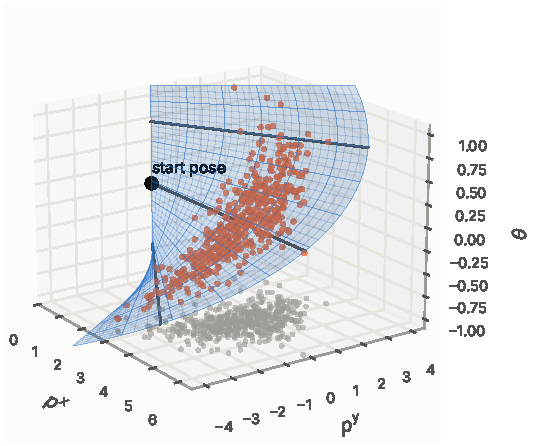
\includegraphics[width=0.72\linewidth]{figures/ch01_helicoid.pdf}
\caption{The poses reachable in one step from the start pose (black dot),
with the noise exaggerated for visibility ($\sigma_s=0.6$,
$\sigma_\delta=0.35$\,rad). Orange: 500 sampled poses $(p^x,p^y,\theta)$;
they all lie on a helicoid (blue), whose horizontal slices are the
straight segments of fixed heading (dark lines). Grey: their shadow on
the lawn, the positions alone, an arc-shaped band.}
\label{fig:helicoid}
\end{figure}

With the real noise of the simulations ($\sigma_s=0.4$,
$\sigma_\delta=0.03$), one step covers only a small patch of the
staircase, which looks almost flat. The curvature becomes visible as the
steps accumulate.

\begin{figure}[ht]
\centering
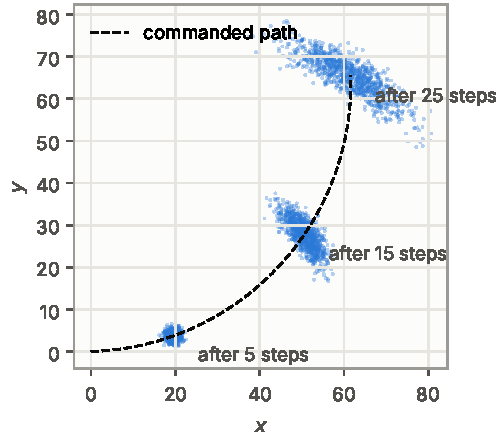
\includegraphics{figures/ch01_transition.pdf}
\caption{A thousand mowers start at the origin, heading east, and receive
the same 25 commands (drive 4, turn $\pi/50$). Their positions after 5,
15 and 25 steps. Only the positions are plotted: each cloud is the shadow
on the lawn of a cloud in the three-dimensional pose space, which after
several steps fills a curved volume rather than a single helicoid. Heading
errors become position errors \emph{across} the path, along arcs: the
clouds bend.}
\label{fig:transition}
\end{figure}

\section{Sensors}

Angles need one piece of notation. All headings and bearings are kept in
$[-\pi,\pi)$ by
\[
  \wrap(a)=a+2\pi k\quad\text{with the unique }k\in\mathbb{Z}\text{ such
  that }a+2\pi k\in[-\pi,\pi).
\]

\begin{lemma}{Angle differences}{wrap}
For angles $a,b$, $\wrap(a-b)$ is the signed rotation of smallest
magnitude that takes $b$ to $a$, and $\wrap(a-b)=\wrap(\wrap(a)-\wrap(b))$.
The plain difference $a-b$ of two wrapped angles can be off by $\pm2\pi$.
\end{lemma}

\begin{proof}
The rotations taking $b$ to $a$ are $a-b+2\pi k$, $k\in\mathbb{Z}$; exactly
one lies in $[-\pi,\pi)$, and it has the smallest magnitude (up to the tie
at $\pm\pi$). Since $\wrap(a)-a$ and $\wrap(b)-b$ are multiples of $2\pi$,
so is their difference, which $\wrap$ removes. For the last claim take
$a=3.10$ and $b=-3.12$: $a-b=6.22$, whereas $\wrap(a-b)=-0.063$.
\end{proof}

\begin{definition}{Range--bearing sensor}{rb}
The lawn holds $M$ landmarks (beacons) at known positions
$\bell_1,\dots,\bell_M$. For landmark $j$ let $\vect{d}=\bell_j-\p$, where
$\p=(p^x,p^y)$. The sensor returns
\begin{equation}\label{eq:h}
  \z_{t,j}=h_j(\x_t)+\vv_{t,j},\qquad
  h_j(\x)=\begin{pmatrix}\norm{\vect{d}}\\
  \wrap\bigl(\operatorname{atan2}(d_y,d_x)-\theta\bigr)\end{pmatrix},
  \qquad \vv_{t,j}\sim\Normal\bigl(\vect0,\,R_1\bigr),
\end{equation}
$R_1=\diag(\sigma_r^2,\sigma_\phi^2)$, for the landmarks within range,
with all $\vv_{t,j}$ independent. The bearing is measured \emph{relative to
the heading}, so it carries information about $\theta$.
\end{definition}

\begin{figure}[ht]
\centering
\begin{tikzpicture}[scale=1.4,>=Stealth,
    mower/.style={draw=black!80,fill=green!35,line width=0.5pt}]
  \coordinate (P) at (0,0);
  \coordinate (L) at (3.6,2.1);
  \def\th{12}
  \draw[dashed,black!45] (P) -- ++(2.4,0) node[right,black!60]
    {\small $x$-direction};
  \draw[dashed,black!45] (P) -- ++(\th:4.3) node[right,black!60]
    {\small heading};
  \draw[->,black!80] (P) ++(0:1.75) arc[start angle=0,end angle=\th,
    radius=1.75];
  \node at ($(P)+({\th/2}:2.0)$) {$\theta$};
  \draw[very thick,orange!85!black] (P) -- (L)
    node[midway,above left] {$r=\norm{\bell_j-\p}$};
  \draw[->,blue!70!black,thick] (P) ++(\th:1.2) arc[start angle=\th,
    end angle={atan2(2.1,3.6)},radius=1.2];
  \node[blue!70!black] at ($(P)+({(\th+atan2(2.1,3.6))/2}:1.42)$) {$\phi$};
  \begin{scope}[shift={(P)},rotate=\th]
    \draw[mower] (-0.32,-0.2) -- (0.2,-0.2) -- (0.32,-0.08) -- (0.32,0.08)
      -- (0.2,0.2) -- (-0.32,0.2) -- cycle;
    \fill[black!80] (0,0) circle (0.035);
  \end{scope}
  \node[below=8pt] at (P) {$\p=(p^x,p^y)$};
  \node[star,star points=5,fill=black!70,inner sep=1.6pt] at (L) {};
  \node[above right] at (L) {landmark $\bell_j$};
\end{tikzpicture}
\caption{The range--bearing measurement of landmark $j$. The range $r$ is
the distance from the mower to the landmark; the bearing $\phi$ is the
angle from the mower's heading to the line of sight, so that the direction
of the landmark in the lawn's frame is $\theta+\phi$.}
\label{fig:sensor}
\end{figure}

\Cref{fig:sensor} shows the two components of $h_j$.

Two simpler sensors are used in Chapters~\ref{ch:bayes}
and~\ref{ch:kalman}: a \emph{GPS-like position fix}
$\z_t=\p_t+\vv_t$, $\vv_t\sim\Normal(\vect0,\sigma_{\mathrm{gps}}^2I)$, and
a \emph{compass} $c_t=\wrap(\theta_t+\nu_t)$,
$\nu_t\sim\Normal(0,\sigma_c^2)$.

A last question is whether the sensor says \emph{which} landmark it saw.
When it does (\emph{known data association}) the measurement is the
indexed family $(\z_{t,j})_j$. When it does not, it is only the set of
$(r,\phi)$ pairs, and the filter must work out the correspondence itself
(\cref{sec:ekf-association,sec:pf-association}).

\section{The two assumptions}

\begin{definition}{Markov state and conditionally independent measurements}{markov}
\begin{enumerate}[label=(A\arabic*),nosep]
\item\label{A1} \emph{Markov motion}: given $\x_{t}$ and $\uu_t$, the
  next state is independent of all earlier states, controls and
  measurements:
  $p(\x_{t+1}\mid\x_{0:t},\uu_{0:t},\z_{1:t})=p(\x_{t+1}\mid\x_t,\uu_t)$.
\item\label{A2} \emph{Conditionally independent measurements}: given
  $\x_t$, the measurement $\z_t$ is independent of everything else:
  $p(\z_t\mid\x_{0:t},\uu_{0:t-1},\z_{1:t-1})=p(\z_t\mid\x_t)$.
\end{enumerate}
\end{definition}

Indices follow the code: control $\uu_t$ moves the mower from $\x_t$ to
$\x_{t+1}$, and $\z_{t+1}$ is measured at $\x_{t+1}$. Both assumptions
hold for the model above by construction, since the noises
$\bepsilon_t$ and $\vv_t$ are independent of everything else.

\begin{proposition}{Factorisation of the joint distribution}{joint}
Under \ref{A1}--\ref{A2}, for known controls $\uu_{0:T-1}$,
\begin{equation}\label{eq:joint}
  p(\x_{0:T},\z_{1:T}\mid\uu_{0:T-1})=p(\x_0)\prod_{t=0}^{T-1}
  p(\x_{t+1}\mid\x_t,\uu_t)\,p(\z_{t+1}\mid\x_{t+1}).
\end{equation}
\end{proposition}

\begin{proof}
Order the variables as $\x_0,\x_1,\z_1,\x_2,\z_2,\dots$ and apply the
chain rule of probability, conditioning each variable on all the previous
ones (and on the controls). The factor of $\x_{t+1}$ is
$p(\x_{t+1}\mid\x_{0:t},\z_{1:t},\uu_{0:T-1})$. Future controls carry no
information about the past motion (they are chosen in advance or from
past data), so this equals $p(\x_{t+1}\mid\x_{0:t},\z_{1:t},\uu_{0:t})$,
which is $p(\x_{t+1}\mid\x_t,\uu_t)$ by \ref{A1}. The factor of
$\z_{t+1}$ is $p(\z_{t+1}\mid\x_{0:t+1},\z_{1:t},\uu)$, which is
$p(\z_{t+1}\mid\x_{t+1})$ by \ref{A2}.
\end{proof}

\begin{inwords}
The whole story, every pose and every measurement, is a chain of small
local pieces: a start, then alternately ``move'' and ``look''. The state
is a sufficient summary of the past: once you know where the mower is,
how it got there is irrelevant to what happens next. That is exactly what
makes a \emph{recursive} filter possible, one that keeps only a belief
about the current state.
\end{inwords}

The densities in \eqref{eq:joint} are a convenient notation. By
\cref{prop:degenerate} the transition has no density on $\R^3$; the
identities in this book remain true with $p(\x_{t+1}\mid\x_t,\uu_t)$ read
as a transition \emph{kernel}, integrals as integrals against it. The
particle filter (\cref{ch:particle}) never needs the density at all: it
only \emph{samples} the motion.

\section{Why filter? Dead reckoning}

The simplest estimator ignores the sensors and integrates the commands:
$\hx_{t+1}=f(\hx_t,\uu_t)$ from the known start. This is \emph{dead
reckoning}. Its error is driven by the control noise, and grows without
bound.

\begin{proposition}{Dead-reckoning error on a straight path}{deadreckoning}
Let the mower start at a known pose heading along the $x$-axis and receive
$t$ commands $\uu=(s,0)$. Let $e_t=p^y_t$ be its lateral error and
$a_t=st-p^x_t$ its forward shortfall with respect to dead reckoning. Then
\begin{align}
  \theta_t&=\textstyle\sum_{k=1}^t\varepsilon_{\delta,k},
  & \Var(\theta_t)&=t\,\sigma_\delta^2,\label{eq:drheading}\\
  e_t&\approx s\textstyle\sum_{k=1}^t\theta_k,
  & \Var(e_t)&\approx s^2\sigma_\delta^2\,\frac{t(t+1)(2t+1)}{6},
  \label{eq:drlateral}\\
  \E[a_t]&\approx\frac{s\,\sigma_\delta^2}{4}\,t(t+1),
  \label{eq:drshort}
\end{align}
where $\approx$ means up to terms of higher order in the noise standard
deviations.
\end{proposition}

\begin{proof}
Heading errors simply add up, so $\theta_t$ is a sum of $t$ independent
$\Normal(0,\sigma_\delta^2)$ variables, which gives \eqref{eq:drheading}.
At step $k$ the mower moves by $(s+\varepsilon_{s,k})(\cos\theta_k,
\sin\theta_k)$. Its lateral component is $(s+\varepsilon_{s,k})
\sin\theta_k=s\theta_k+O(\varepsilon^2)$, so
$e_t\approx s\sum_k\theta_k=s\sum_{k=1}^t\sum_{j=1}^k\varepsilon_{\delta,j}
=s\sum_{j=1}^t(t-j+1)\varepsilon_{\delta,j}$. The variance of a sum of
independent terms is the sum of the variances:
$s^2\sigma_\delta^2\sum_{m=1}^t m^2$, which is \eqref{eq:drlateral}.
The forward displacement at step $k$ is
$(s+\varepsilon_{s,k})\cos\theta_k=s+\varepsilon_{s,k}-\tfrac s2\theta_k^2
+O(\varepsilon^3)$, so $\E[a_t]\approx\tfrac s2\sum_k\E[\theta_k^2]=
\tfrac s2\sigma_\delta^2\sum_k k$.
\end{proof}

\begin{inwords}
The lateral error grows like $t^{3/2}$, not like $\sqrt t$: each heading
error is \emph{integrated} along the rest of the path. Worse, the mower is
\emph{on average} short of where dead reckoning puts it, because a wrong
heading always shortens the forward progress. That bias, the
$\E[\cos\theta]<1$ effect, is invisible to any method that linearises the
motion, and will reappear in Chapter~\ref{ch:ekf}.
\end{inwords}

With the noise of the simulations ($s=4$, $\sigma_\delta=0.03$) and
$t=100$, \eqref{eq:drlateral} predicts a lateral standard deviation of
$69.8$ and \eqref{eq:drshort} a shortfall of $9.1$. A Monte Carlo run with
20\,000 mowers gives $67.5$ and $8.9$. On the figure-eight path of the
simulations the loops partly cancel the error (rotating a closed loop about
its start leaves its end in place), and the median error after 100 steps is
about 21; but it still grows without bound
(\cref{fig:deadreckoning}).

\begin{figure}[ht]
\centering
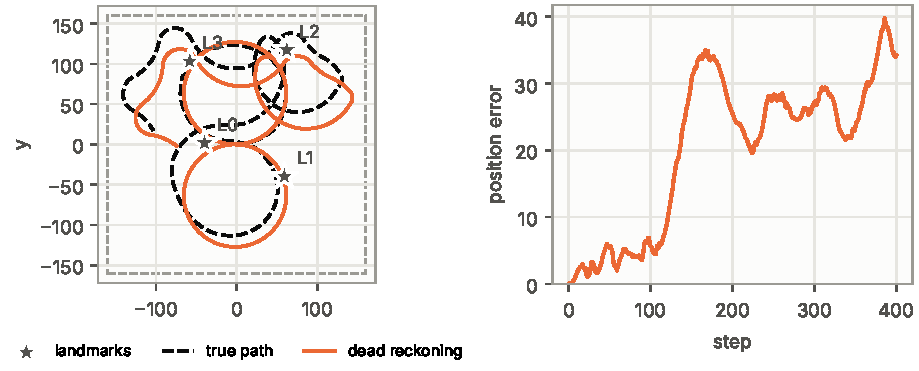
\includegraphics[width=\linewidth]{figures/ch01_dead_reckoning.pdf}
\caption{Dead reckoning on the standard run (seed 1). Left: the true path
and the integrated commands. Right: the position error. It is a random
walk, and nothing pulls it back.}
\label{fig:deadreckoning}
\end{figure}

A single GPS fix has the opposite problem: its error never grows, but it
never shrinks either (an RMS of $\sigma_{\mathrm{gps}}\sqrt2\approx11$ with
$\sigma_{\mathrm{gps}}=8$). A \emph{filter} combines the two: it uses the
motion model to carry information forward in time, and each new
measurement to correct the drift.

\begin{practice}[\nb{00\_the\_mower\_world.ipynb}, \code{world.py}]
\code{World} holds the lawn, the landmarks and the \emph{true} noise
levels; \code{motion\_model} and \code{range\_bearing} are $f$ and $h$,
vectorised over leading dimensions so that they also move whole clouds
of particles or sigma points. \code{simulate} returns a \code{Run} with the
true poses, the commanded controls and every sensor reading. The pilot of
the simulation steers the mower back towards the centre near the edges of
the lawn; that steering is part of the \emph{command}, so the filters know
it. The notebook draws \cref{fig:transition,fig:deadreckoning}.
\end{practice}

\begin{mower}
On a real mower the control is the odometry reported by the wheel
encoders, not the command sent to the motors, and its noise depends on
the ground: much larger on wet grass or a slope, where the wheels slip.
Those are also the conditions in which the heading error, and therefore
the $t^{3/2}$ growth, is worst. A robot mower that relied on odometry
alone would drift off its stripes within a few metres. This is why every
commercial one has a second source of position: a boundary wire, beacons,
RTK-GNSS or a camera.
\end{mower}

\FloatBarrier
\section*{Exercises}
\addcontentsline{toc}{section}{Exercises}

\begin{enumerate}[label=\textbf{1.\arabic*},ref=1.\arabic*]
\item\label{ex:nullspace} Compute the null space of $Q=VMV\T$ from
  \cref{prop:degenerate}. Which combination of position and heading
  errors can a single step never produce, to first order?
\item\label{ex:ecos} Let $\theta\sim\Normal(0,\sigma^2)$. Show that
  $\E[\cos\theta]=e^{-\sigma^2/2}$ and $\E[\sin\theta]=0$. Deduce the
  exact mean forward progress of one noisy step from a heading known up to
  $\Normal(0,\sigma^2)$, and compare it with the linearised value $s$.
\item\label{ex:condind} Using \cref{prop:joint}, show that the
  measurements are \emph{not} independent of one another, but that they
  are independent given the states: $p(\z_{1:T}\mid\x_{0:T})=
  \prod_t p(\z_t\mid\x_t)$.
\item\label{ex:wrapadd} Is $\wrap$ additive, i.e.\ is
  $\wrap(a+b)=\wrap(a)+\wrap(b)$? Give a proof or a counter-example, and
  explain why the code wraps the heading \emph{after} each update.
\end{enumerate}

\subsection*{Solutions}

\textbf{1.1.} The null space of $VMV\T$ equals the null space of $V\T$
because $M$ is positive definite. A vector $\vect{n}$ with $V\T\vect{n}=
\vect0$ is orthogonal to both columns of $V$, so it is their cross
product:
\[
  \vect{n}=\begin{pmatrix}\cos\theta'\\\sin\theta'\\0\end{pmatrix}\times
  \begin{pmatrix}-s\sin\theta'\\s\cos\theta'\\1\end{pmatrix}
  =\begin{pmatrix}\sin\theta'\\-\cos\theta'\\s\end{pmatrix}.
\]
To first order, the error $\Delta\x$ of one step satisfies
$\vect{n}\T\Delta\x=0$, i.e.\ $\Delta_{\perp}=s\,\Delta\theta$, where
$\Delta_\perp=-\sin\theta'\Delta p^x+\cos\theta'\Delta p^y$ is the
sideways position error: a sideways error can only come from having turned
wrongly, and the two are tied. A sideways jump with the right heading is
impossible.

\textbf{1.2.} $\E[e^{i\theta}]=e^{-\sigma^2/2}$ is the characteristic
function of $\Normal(0,\sigma^2)$ at $1$. Its real and imaginary parts
are $\E[\cos\theta]$ and $\E[\sin\theta]$; the second is also $0$ because
$\sin$ is odd and the distribution symmetric. A step of length $s$ in
direction $\theta$ therefore advances by $s\,e^{-\sigma^2/2}<s$ on
average. Linearising $\cos\theta\approx1$ gives $s$, and the bias
$s(1-e^{-\sigma^2/2})\approx s\sigma^2/2$ is exactly the per-step term in
\eqref{eq:drshort}.

\textbf{1.3.} Integrating \eqref{eq:joint} over $\x_{0:T}$ gives
$p(\z_{1:T}\mid\uu)$, which does not factorise: two measurements both
depend on the trajectory, which is random (two GPS fixes taken one step
apart are strongly correlated because the mower was nearly in the same
place). Dividing \eqref{eq:joint} by $p(\x_{0:T}\mid\uu)=p(\x_0)\prod_t
p(\x_{t+1}\mid\x_t,\uu_t)$, which is the marginal of \eqref{eq:joint}
obtained by integrating out every $\z_t$ (each likelihood integrates to
one), leaves $\prod_t p(\z_t\mid\x_t)$.

\textbf{1.4.} No: $\wrap(3+3)=6-2\pi\approx-0.28$, whereas
$\wrap(3)+\wrap(3)=6$. $\wrap$ is additive only modulo $2\pi$:
$\wrap(a+b)=\wrap(\wrap(a)+\wrap(b))$. A filter update adds a correction
$K\y$ to the heading; the sum may leave $[-\pi,\pi)$, and if it is not
wrapped, the next innovation (a difference of angles,
\cref{lem:wrap}) or the next circular mean will treat a heading of
$3.2$ and one of $-3.08$ as different, although they are the same
direction.
